\documentclass[]{article}
\usepackage[utf8]{inputenc} 
\usepackage[T1]{fontenc}
\usepackage{lmodern}
\usepackage[ngerman]{babel}
\usepackage{courier}
\usepackage{amsmath}
\usepackage{multicol}
\usepackage[top=2cm, bottom=2cm, left=2cm, right=2cm]{geometry}
\usepackage{authblk}
\usepackage[font=scriptsize, labelfont=bf]{caption}
\usepackage{listings}
\usepackage{hyperref}
\usepackage{color}
\usepackage{float}
\usepackage{amssymb}
\usepackage{graphicx, caption}
\usepackage{sidecap}
\usepackage{flafter}  
\usepackage[style=numeric]{biblatex}
\usepackage[babel,german=guillemets]{csquotes}
\usepackage{feynmp-auto}
\bibliography{literatur}
\usepackage{bbm}
\definecolor{dkgreen}{rgb}{0,0.6,0}
\definecolor{gray}{rgb}{0.5,0.5,0.5}
\definecolor{mauve}{rgb}{0.58,0,0.82}


\lstset{frame=tb,
  language=C,
  aboveskip=3mm,
  belowskip=3mm,
  showstringspaces=false,
  columns=flexible,
  basicstyle={\small\ttfamily},
  numbers=none,
  numberstyle=\tiny\color{gray},
  keywordstyle=\color{blue},
  commentstyle=\color{dkgreen},
  stringstyle=\color{mauve},
  breaklines=true,
  breakatwhitespace=true,
  tabsize=3
  }
\captionsetup{width=1\linewidth}

% for skript letters like H...
\usepackage{mathrsfs}
\usepackage{fancyhdr}
\fancyhf{}
\fancyfoot[LE,RO]{\thepage}
\usepackage{hyperref}
\pagestyle{fancy}
\geometry{verbose,a4paper,tmargin=25mm,bmargin=25mm,lmargin=15mm,rmargin=20mm}



\title{Protocol on $Z^0$-decay}

\author{Nicolas Heimann}
\affil{nicolas.heimann@studium.uni-hamburg.de}
\author{Jesse Hinrichsen}
\affil{jesse.hinrichsen@studium.uni-hamburg.de}
\date{07.03. - 12.03.2016}
\affil{Universität Hamburg}
\begin{document}
\begin{titlepage}
\maketitle
\thispagestyle{empty}
\abstract{
An abstract...
}
\end{titlepage}



\tableofcontents
\pagebreak
\section {Introduction}
In this experiment we analyse existing data about the $Z^0$-decay after a $e^-e^+$ collision. Based on Monte-Carlo simulated data and theoretical considerations we define parameter cuts to define different decay channels for the $Z^0$-boson. Applied to a real dataset obtained from the OPAL experiment at CERN we determine cross-section, partial width for different decay channels, as well as the weinberg-angle and compare the results to theoretical values. 

\section{Theory}
The process we are interested is $e^-e^+ \rightarrow f\bar f$. By the Standardmodel this is possible by an exchange of either photon or $Z^0$. Figure \ref{fig:feynman-low} shows the lowest order of Feynman diagrams.

\begin{figure}[H]
	\vspace{1cm}
	\centering


\begin{fmffile}{diagram}

  \begin{fmfgraph*}(100,60)
\fmfleft{i1,i2}
\fmfright{o1,o2}
\fmflabel{$e^-$}{i1}
\fmflabel{$e^+$}{i2}
\fmflabel{$\bar f$}{o1}
\fmflabel{$f$}{o2}

\fmf{vanilla}{i1,v1,i2}
\fmf{vanilla}{o1,v2,o2}
\fmf{photon,label=$\gamma,,Z^0$}{v1,v2}
    
  \end{fmfgraph*}
\hspace{2cm}
    \begin{fmfgraph*}(80,50)
    
    
\fmfleft{i1,o1}
\fmfright{i2,o2}


\fmflabel{$e^-$}{i1}
\fmflabel{$e^-$}{i2}
\fmflabel{$e^+$}{o1}
\fmflabel{$e^+$}{o2}

\fmf{vanilla}{i1,v1,i2}
\fmf{vanilla}{o1,v2,o2}
\fmf{photon,label=$\gamma,,Z^0$}{v1,v2}

    
  \end{fmfgraph*}

\end{fmffile}
	\vspace{1cm}
	\caption{Lowest order Feynman diagrams for $e^-e^+ \rightarrow f\bar f$. Left: S-channel. Right: T-channel, $Z^0$ is possible but very unlikely due to the low masses of the elektron and the high mass of the $Z^0$.}
	\label{fig:feynman-low}
\end{figure}
At $\sqrt{s}=M_{Z^0}$ the probability that $Z^0$ is the propagator for the scattering process is much higher than for the photon.

\subsection{Corrections}
Additional Feynman diagrams have to be taken into account to evaluate the actual properties of the $Z^0$. Thus Bremstrahlung (photon emitted by the elektron before the collision) will shift the $Z_0$ resonance to a higher energy.


\section{Identifying events}
Based on the theory we can calculate the following properties for the different decay channels.

\subsection{Decay width and cross-section}
Using\footnote{equation 2.12 page 18 experiment folder}
\begin{equation}
\Gamma_f = \frac{N^f_c \sqrt{2}}{12 \pi} G_F M_Z^3(g_V^{f2} + g_A^{f2})
\end{equation}
we calculate the decay width and\footnote{equation 2.14 page 18 experiment folder}
\begin{equation}
\sigma^{peak}_f= \frac{12 \pi}{M_Z^2} \frac{\Gamma_e}{\Gamma_Z}\frac{\gamma_f}{\Gamma_Z}
\end{equation}
the cross-section at peak of the Z-boson into fermions\footnote{$\Gamma_{lept}$ is the decay channels without neutrinos}.

\begin{tabular}{ |p{3cm}||p{3cm}|  }
 \hline
 \multicolumn{2}{|c|}{Decay width for different channels} \\
 \hline
 Channel & Decay width \\
 \hline
  $\Gamma_l = \Gamma_e = \Gamma_{\mu} = \Gamma{\tau} $   & 85.9 MeV   \\
  $\Gamma_{\nu} $   & 165.9 MeV   \\
  $\Gamma_u = \Gamma_c $   & 301.5 MeV   \\
  $\Gamma_d = \Gamma_s = \Gamma_b $   & 381.4 MeV   \\
  \hline
  $\Gamma_Z $   & 2502.7 MeV   \\
  $\Gamma_{hadr} $   & 1747.3 MeV   \\
  $\Gamma_{lept} $   & 257.8  MeV   \\
  $\Gamma_{neutr} $   & 497.6  MeV   \\
 \hline
 \hline
 \multicolumn{2}{|c|}{Partial cross-section at peak} \\
 \hline
  $\sigma_{lept} $   & 5.35 $KeV^{-2}$   \\
  $\sigma_{neutr} $   & 10.32 $KeV^{-2}$   \\
  $\sigma_{u, c} $   & 18.76 $KeV^{-2}$   \\
  $\sigma_{d,s,c} $   & 23.73 $KeV^{-2}$   \\
 \hline
\end{tabular}

\subsection{Estimating change of $Z^0$ decay width for additional channels}
If we take additional decay channels into account, thus assuming more lepton and quark generations we calculate the following increase of the decay width.

\begin{tabular}{ |p{3cm}||p{3cm}|p{3cm}|  }
 \hline
 \multicolumn{3}{|c|}{Decay width of $Z^0$ for additional channels} \\
 \hline
 Added channel & $Z^0$ width & relative increase \\
 \hline
   Lepton & 2.589 GeV & 3.5 \%  \\
   Neutrino & 2.669  GeV & 6.6 \%  \\
   u-Quark & 2.804  GeV & 12 \%  \\
   d-Quark & 2.884 GeV & 15.2 \%  \\
  \hline
\end{tabular}

\subsection{Differential cross-section}
As mentioned above we also have to take the t-channel decay into account. For the differential cross-section the following proportionalities differentiate between the channels
\newline
S-channel: $\frac{d\sigma}{d\Omega} \propto 1 + \cos^2{\Theta}$ (for big $\Theta$)
\newline
T-channel: $\frac{d\sigma}{d\Omega} \propto (1 - \cos{\Theta})^{-2}$ (for small $\Theta$)
\begin{figure}[H]
	\centering
	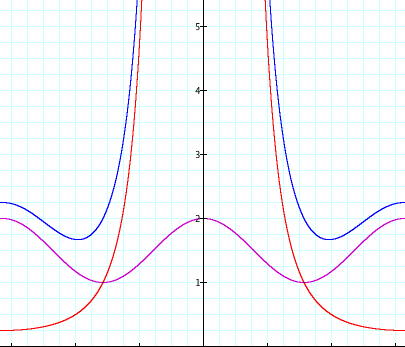
\includegraphics[scale=0.4]{differential-cross-section}
	\hspace{3cm}
	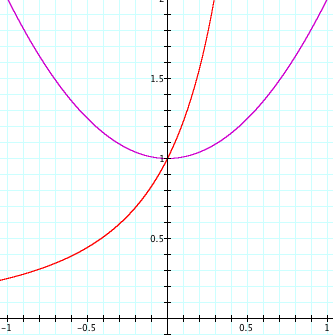
\includegraphics[scale=0.4]{cross-section-diff}
	
	\caption{Differential cross-section on $\Theta$ (left), differential cross-section on $\cos{\Theta}$ (right) qualitatively. Red: t-channel, violet: s-channel, blue: s-channel + t-channel. Right: }
	\label{fig:diff-cross-section}
\end{figure}
For the $e^-e^+ \rightarrow e^-e^+$ we have to evaluate events in the area $-1 \leq \cos{\Theta} \leq 0$, since we are only interested in the $Z^0$ as propagator. In section 4 we will make a better estimation to distinguish s from t-channel.

\subsection{Forward-Backward Asymmetry}
Based the equation\footnote{equation 2.18 page 19 experiment folder} for the forward-backward asymmetry, we calculate the following factors

\begin{tabular}{ |p{3cm}||p{2cm}|p{2cm}|p{2cm}|  }
 \hline
 \multicolumn{4}{|c|}{Forward-Bckward asymmetry} \\
 \hline
 $\sqrt{s}$ / $\sin^2(\theta_W)$ & 0.21 & 0.23 & 0.25 \\
 \hline
   89.225 GeV & 0.547 & 0.321 & 0.285  \\
   91.225 GeV & 0.530 & 0.407 & 0.284  \\
   93.225 GeV & 0.515 & 0.480 & 0.284  \\
  \hline
\end{tabular}

If we plot the forward-backward asymmetry against $\sin^2(\theta_W)$ and $\sqrt{s}$, we get a distribution as in figure \ref{fig:for-back-asy}
\begin{figure}[H]
	\centering
	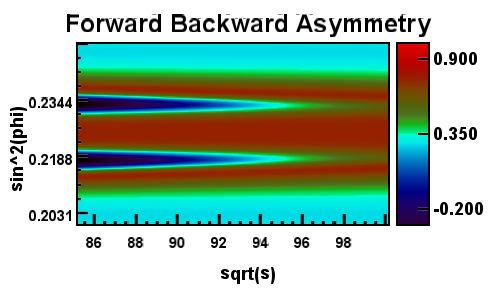
\includegraphics[scale=0.6]{forward_backward_symmetry}
	\caption{Forward-Backward asymmetry}
	\label{fig:for-back-asy}
\end{figure}

\section{Analyzing data}
We now use simulated data for specific events to find parameter cuts. With those cuts we will then be able to identify the decay channels for a set of real data.

\subsection{Monte-Carlo data}
Using the monte-carlo data we define the following cuts\footnote{x defines either the lowest or highest possible value} to distinguish different event types.

\begin{tabular}{ |p{4cm}||p{2cm}|p{2cm}|p{2cm}|p{2cm}|  }
 \hline
 CUT & e & $\tau$ & $\mu$ & q \\
 \hline
 ECAL lower & 85 & 0 & 8 & 15 \\
 ECAL upper & 100 & 30 & 75 & x \\
 HCAL lower & x & 0 & x & x \\
 HCAL upper & x & 20 & x & x \\
 PCHARGED lower & x & 70 & 8 & x \\
 PCHARGED upper & x & x & 58 & x \\
 N lower & x & x & 2 & 7 \\
 N upper & x & 4 & 7 &x \\
 $\cos\theta_1$ lower & -0,7 & x & x & x \\
 $\cos\theta_1$ upper & -0,188342 & x & x & x \\
 $\cos\theta_2$ lower & x & x & x & x \\
 $\cos\theta_2$ upper & x & x & x & x \\
 \hline
\end{tabular}
\newline
ECAL: Energy in electronic-kalorimeter
\newline
HCAL: Energy in hadronic-kalorimeter
\newline
PCHARGED: Momentum of all charged traces
\newline
N: Number of charged traces
\newline
$\theta$: Angle of distribution along the z-axis
\newline
\newline
Thereby we already separated the s from the t-channel based on the following calculation
\newline
We want to find $\cos\theta$ so that we filter most t-channel events:
\begin{equation}
\frac{T}{T+S} \leq 0.05
\label{eq:cond}
\end{equation}
where  $T=a(1-\cos{\theta})^{-2}$  and $S=b(1+\cos^2{\theta})$. 
The differential crossection is then
\begin{equation}
\frac{dN}{d\cos\theta} = \frac{a}{(1-\cos\theta)^2}+b(1+\cos^2\theta)
\end{equation}
where we integrate over $\cos\theta$.
\begin{equation}
\int dN = \frac{a}{1-\cos\theta} + b\left(\cos\theta+\frac{1}{3}\cos^3\theta\right)
\end{equation}
We obtain detector errors outside $cos\theta \in [-0.7,0.7]$. Therefore the integration is performed only on that interval. Since we have two unkowns in the equation we split the integral into two integrals to get two linear equation:
\begin{equation}
\begin{split}
11786 &= a(\frac{1}{1-0.7}-1)+b(0,7+\frac{1}{3}0.7^3) =  (2+\frac{1}{3})a+0,813433b\\
9620 &= a(1-\frac{1}{1+0.7})+b(0,7+\frac{1}{3}0.7^3) = 0,4117647a+ 0,813433b\\
\end{split}
\end{equation}
With the power of basic linear algebra we get $a=1127,2$ and $b=9155,857$.
We can now compute the true number of events in s-channel:
\begin{equation}
N_s = b\int_{-1}^1 d\cos\theta (1+\cos^2\theta) = \frac{8}{3}b = 24413
\end{equation}
Insert a and b into condition (\ref{eq:cond}) we get a upper boundary for $\cos\theta$
\begin{equation}
\frac{a}{(1-\cos\theta)^2}\frac{1}{\frac{a}{(1-\cos\theta)^2}+b(1+\cos^2\theta))} \leq 0.05 \iff \cos\theta \leq -0.188342
\end{equation}
For the given cuts we find the the following number of events
\newline
\newline
\begin{tabular}{ |p{3cm}||p{2cm}|p{2cm}|p{2cm}|p{2cm}|  }
 \hline
 Type / Events & e & $\tau$ & $\mu$ & q \\
 \hline
  ELECTRON & 6980 & 1 & 0 & 0 \\
  MUON & 0 & 86598 & 457 & 0 \\
  TAU & 286 & 723 & 62832 & 399 \\
  HADRONS & 25 & 0 & 949 & 97980 \\
 \hline
\end{tabular}
\newline
\newline
If no filter applied we get the following event ratios based on the fact that each set of simulated data has 100000 events. 
\newline
\newline
\begin{tabular}{ |p{3cm}||p{2cm}|p{2cm}|p{2cm}|p{2cm}|  }
 \hline
 Events & e & $\tau$ & $\mu$ & q \\
 \hline
 \hline
  TOTAL & 89719 & 94339 & 79191 & 98501 \\
  \hline
  RATIO & 1,115 & 1,06 & 1,263 & 1,015 \\
 \hline
\end{tabular}
\newline
\newline
Now we can calculate the efficiency matrix $\epsilon$, where each element is defined as 
\begin{equation}
\epsilon_{i,j} = \frac{N_{cut}}{N_{true}}
\end{equation}
\begin{equation}
\epsilon=\begin{pmatrix}
   2.86\cdot 10^{-01} & 1.0\cdot 10^{-05} & 0 & 0 \\
   0 & 9.18\cdot 10^{-01} & 5.77\cdot 10^{-03} & 0 \\
   3.03\cdot 10^{-03} & 9.13\cdot 10^{-03} & 7.93\cdot 10^{-01} & 4.05\cdot 10^{-03} \\
   1.02\cdot 10^{-03} & 0 & 1.2\cdot 10^{-02} & 9.95\cdot 10^{-01} \\
\end{pmatrix}
\end{equation}
With $N_{true} = \epsilon^{-1} N_{obs}$ we are now able to obtain the true number of events.
\begin{equation}
\epsilon^{-1}=\begin{pmatrix}
   3.5 & -3.81\cdot 10^{-05} & 2.77\cdot 10^{-07} & -1.13\cdot 10^{-09} \\
   8.39\cdot 10^{-05} & 1.09 & -7.92\cdot 10^{-03} & 3.23\cdot 10^{-05} \\
   -1.33\cdot 10^{-02} & -1.25\cdot 10^{-02} & 1.26 & -5.13\cdot 10^{-03} \\
   -3.43\cdot 10^{-03} & 1.51\cdot 10^{-04} & -1.52\cdot 10^{-02} & 1.01 \\
\end{pmatrix}
\end{equation}
The uncertainty matrix can be calculated using
\begin{equation}
\Delta \epsilon = \sqrt{\frac{\epsilon(1-\epsilon)}{N}}
\end{equation}
and with
\begin{equation}
\epsilon\Delta\epsilon^{-1}+\Delta\epsilon\epsilon^{-1}=0
\end{equation}
we get the uncertainty matrix for $\epsilon^-1$
\begin{equation}
\Delta\epsilon^{-1} = -\epsilon^{-1}\Delta\epsilon\epsilon^{-1} = \begin{pmatrix}
   -3.55 \cdot 10^{-02} & 4.24 \cdot 10^{-07} & 1.08 \cdot 10^{-08} & -9.96 \cdot 10^{-11} \\
   1.43 \cdot 10^{-05} & -1.06 \cdot 10^{-03} & -3.9 \cdot 10^{-04} & 3.18 \cdot 10^{-06} \\
   -1.6 \cdot 10^{-03} & -3.78 \cdot 10^{-04} & -2.21 \cdot 10^{-03} & -2.43 \cdot 10^{-04} \\
   -6.42 \cdot 10^{-04} & 9.57 \cdot 10^{-06} & -4.77 \cdot 10^{-04} & -1.97 \cdot 10^{-04} \\
\end{pmatrix}
\end{equation}

\subsection{OPAL data}
Now we apply above cuts to dataset 4 from the OPAL experiment.

\subsection{Pure Events}
For the $e^+, e^-$ detection we have to apply a cut for the $-0.71 \leq \cos(\theta) \leq 0.65$ and  $-0.925 \leq \cos(\theta) \leq -0.85$ due to a problem in the detector.
\newline







\subsection{Dataset4}
Apply the cuts we used within monte carlo simulation we could find the total number of observed events for each $\sqrt{s} \in \{88.47939, 89.46793, 90.22266, 91.22430, 91.96648, 92.96465, 93.71712\}$:
\begin{equation}
N_{obs}=\begin{pmatrix}
   2.0\cdot 10^{+01} & 9.0\cdot 10^{+01} & 1.0\cdot 10^{+02} & 2.0\cdot 10^{+03} \\
   8.0\cdot 10^{+01} & 3.0\cdot 10^{+02} & 3.0\cdot 10^{+02} & 7.0\cdot 10^{+03} \\
   9.0\cdot 10^{+01} & 4.0\cdot 10^{+02} & 3.0\cdot 10^{+02} & 9.0\cdot 10^{+03} \\
   6.0\cdot 10^{+02} & 3.0\cdot 10^{+03} & 2.0\cdot 10^{+03} & 7.0\cdot 10^{+04} \\
   1.0\cdot 10^{+02} & 6.0\cdot 10^{+02} & 5.0\cdot 10^{+02} & 1.0\cdot 10^{+04} \\
   4.0\cdot 10^{+01} & 3.0\cdot 10^{+02} & 3.0\cdot 10^{+02} & 6.0\cdot 10^{+03} \\
   6.0\cdot 10^{+01} & 3.0\cdot 10^{+02} & 3.0\cdot 10^{+02} & 7.0\cdot 10^{+03} \\
\end{pmatrix}
\end{equation}
Where each roch represents one CMS-energy.
Using the inverse efficiency matrix (\ref{eq:eff-inv}) we get true number of events
\begin{equation}
N_{true} = (\epsilon^{-1}N_{obs}^T)^T = \begin{pmatrix}
   6.995\cdot 10^{+01} & 1.006\cdot 10^{+02} & 1.08\cdot 10^{+02} & 2.512\cdot 10^{+03} \\
   2.833\cdot 10^{+02} & 3.053\cdot 10^{+02} & 2.966\cdot 10^{+02} & 6.682\cdot 10^{+03} \\
   3.183\cdot 10^{+02} & 4.214\cdot 10^{+02} & 3.838\cdot 10^{+02} & 8.812\cdot 10^{+03} \\
   2.207\cdot 10^{+03} & 3.12\cdot 10^{+03} & 2.635\cdot 10^{+03} & 6.718\cdot 10^{+04} \\
   3.987\cdot 10^{+02} & 6.252\cdot 10^{+02} & 5.346\cdot 10^{+02} & 1.306\cdot 10^{+04} \\
   1.294\cdot 10^{+02} & 2.847\cdot 10^{+02} & 2.805\cdot 10^{+02} & 6.287\cdot 10^{+03} \\
   1.959\cdot 10^{+02} & 3.163\cdot 10^{+02} & 2.812\cdot 10^{+02} & 7.016\cdot 10^{+03} \\
\end{pmatrix}
\end{equation}
with error of 
\begin{equation}
\Delta N_{true} = \begin{pmatrix}
   -7.095\cdot 10^{-01} & -1.284\cdot 10^{-01} & -8.901\cdot 10^{-01} & -5.511\cdot 10^{-01} \\
   -2.873 & -3.809\cdot 10^{-01} & -2.443 & -1.487 \\
   -3.228 & -5.185\cdot 10^{-01} & -3.19 & -1.948 \\
   -2.238\cdot 10^{+01} & -3.771 & -2.367\cdot 10^{+01} & -1.47\cdot 10^{+01} \\
   -4.044 & -7.586\cdot 10^{-01} & -4.633 & -2.861 \\
   -1.313 & -3.568\cdot 10^{-01} & -2.236 & -1.375 \\
   -1.987 & -3.866\cdot 10^{-01} & -2.463 & -1.531 \\
\end{pmatrix}
\end{equation}
Next we calculate crossection by using equation (S-3.3):
\begin{equation}
\frac{dN}{dt} = \mathcal{L}\sigma
\label{eq:cs}
\end{equation}
Using the following matrix for Strahlungskorrektur from table 5.5
\begin{equation}
\Lambda = \begin{pmatrix}
   9.0\cdot 10^{-02} & 9.0\cdot 10^{-02} & 9.0\cdot 10^{-02} & 2.0 \\
   2.0\cdot 10^{-01} & 2.0\cdot 10^{-01} & 2.0\cdot 10^{-01} & 4.3 \\
   3.6\cdot 10^{-01} & 3.6\cdot 10^{-01} & 3.6\cdot 10^{-01} & 7.7 \\
   5.2\cdot 10^{-01} & 5.2\cdot 10^{-01} & 5.2\cdot 10^{-01} & 1.08\cdot 10^{+01} \\
   2.2\cdot 10^{-01} & 2.2\cdot 10^{-01} & 2.2\cdot 10^{-01} & 4.7 \\
   -1.0\cdot 10^{-02} & -1.0\cdot 10^{-02} & -1.0\cdot 10^{-02} & -2.0\cdot 10^{-01} \\
   -8.0\cdot 10^{-02} & -8.0\cdot 10^{-02} & -8.0\cdot 10^{-02} & -1.6 \\
\end{pmatrix}
\end{equation}
And the following Luminosities given by table 5.6:
\begin{equation}
\mathcal{L}dt = \begin{pmatrix}
   4.6398\cdot 10^{+02} \\
   6.6752\cdot 10^{+02} \\
   4.8676\cdot 10^{+02} \\
   2.2466\cdot 10^{+03} \\
   5.3591\cdot 10^{+02} \\
   4.506\cdot 10^{+02} \\
   7.097\cdot 10^{+02} \\
\end{pmatrix}
\end{equation}
Also we include monte carlo correction factor
\begin{equation}
\mathcal{M} = \begin{pmatrix}
  4.0961279303 \\
  1.060006996 \\
  1.2627697592 \\
  1.0152181196
\end{pmatrix}
\end{equation}
So calculate the crossection for each element $\sigma_{ij} = \mathcal{M}_{j}N_{true,ij}/(\mathcal{L}dt)_i+\Lambda_{ij}$:
\begin{equation}
\sigma = \begin{pmatrix}
   2.66565\cdot 10^{-01} & 3.02468\cdot 10^{-01} & 3.53996\cdot 10^{-01} & 7.47017 \\
   6.97041\cdot 10^{-01} & 6.47807\cdot 10^{-01} & 7.03198\cdot 10^{-01} & 1.44138\cdot 10^{+01} \\
   1.12577 & 1.20711 & 1.255 & 2.59911\cdot 10^{+01} \\
   1.67049 & 1.87841 & 1.86789 & 4.10152\cdot 10^{+01} \\
   1.09134 & 1.36129 & 1.36046 & 2.93176\cdot 10^{+01} \\
   3.26344\cdot 10^{-01} & 6.0869\cdot 10^{-01} & 6.93407\cdot 10^{-01} & 1.38972\cdot 10^{+01} \\
   2.43212\cdot 10^{-01} & 3.56132\cdot 10^{-01} & 3.73723\cdot 10^{-01} & 8.3877 \\
\end{pmatrix}
\end{equation}
The error of cross section in eq (\ref{eq:cs}) is given by
\begin{equation}
\Delta\sigma = \sqrt{\left(\frac{\partial\sigma}{\partial N_{True}}\Delta N_{True}\right)^2+
\left(\frac{\partial\sigma}{\partial (\mathcal{L}dt)}\Delta{\mathcal{L}dt}\right)^2} = \sqrt{\left(\frac{1}{\mathcal{L}dt}\Delta N_{True}\right)^2
+\left(-\frac{N_{True}}{(\mathcal{L}dt)^2}\Delta\mathcal{L}dt\right)^2}
\end{equation}
Where the error of $\mathcal{L}dt$ is given by
\begin{equation}
\Delta\mathcal{L}dt = \pm \begin{pmatrix}
   4.249604 \\
   5.691792 \\
   4.454466 \\
   16.43293 \\
   4.848926 \\
   4.276552 \\
   6.104764 \\
\end{pmatrix} [nb^{-1}]
\end{equation}
Finally we get
\begin{equation}
\Delta\sigma=\begin{pmatrix}
   2.0603\cdot 10^{-03} & 2.0057\cdot 10^{-03} & 2.8681\cdot 10^{-03} & 4.96\cdot 10^{-02} \\
   5.6236\cdot 10^{-03} & 3.9419\cdot 10^{-03} & 5.2671\cdot 10^{-03} & 8.5376\cdot 10^{-02} \\
   8.9322\cdot 10^{-03} & 7.9929\cdot 10^{-03} & 9.747\cdot 10^{-03} & 1.6571\cdot 10^{-01} \\
   1.2284\cdot 10^{-02} & 1.0296\cdot 10^{-02} & 1.3589\cdot 10^{-02} & 2.1885\cdot 10^{-01} \\
   1.0112\cdot 10^{-02} & 1.065\cdot 10^{-02} & 1.2499\cdot 10^{-02} & 2.2052\cdot 10^{-01} \\
   3.9891\cdot 10^{-03} & 6.0496\cdot 10^{-03} & 7.716\cdot 10^{-03} & 1.3245\cdot 10^{-01} \\
   3.6702\cdot 10^{-03} & 3.8727\cdot 10^{-03} & 4.8643\cdot 10^{-03} & 8.506\cdot 10^{-02} \\
\end{pmatrix}
\end{equation}
If we addup first three columns of the matrix we get:
\begin{equation}
\sigma=
\begin{pmatrix}
   7.2261\cdot 10^{-01} & 7.3882 \\
   1.5423 & 1.4262\cdot 10^{+01} \\
   2.7749 & 2.5717\cdot 10^{+01} \\
   4.1898 & 4.0562\cdot 10^{+01} \\
   2.8525 & 2.8949\cdot 10^{+01} \\
   1.1928 & 1.3686\cdot 10^{+01} \\
   6.0966\cdot 10^{-01} & 8.238 \\
\end{pmatrix}
\end{equation}
with an error of
\begin{equation}
\Delta\sigma=
\begin{pmatrix}
   6.9341\cdot 10^{-03} & 4.96\cdot 10^{-02} \\
   1.4833\cdot 10^{-02} & 8.5376\cdot 10^{-02} \\
   2.6672\cdot 10^{-02} & 1.6571\cdot 10^{-01} \\
   3.6169\cdot 10^{-02} & 2.1885\cdot 10^{-01} \\
   3.3262\cdot 10^{-02} & 2.2052\cdot 10^{-01} \\
   1.7755\cdot 10^{-02} & 1.3245\cdot 10^{-01} \\
   1.2407\cdot 10^{-02} & 8.506\cdot 10^{-02} \\
\end{pmatrix}
\end{equation}
Where we used that $\Delta\sum_i a_i=\sqrt{\sum a_i^2}$, while $a_i$ are the partial errors.


\section{Lepton universality}
At high energy equal rights of all families <=> same total cross section

\pagebreak
\nocite{*}
\printbibliography



\end{document}